\documentclass[a4paper,11pt]{report}
 
% Import des extensions
\usepackage[T1]{fontenc}
\usepackage[utf8]{inputenc}
\usepackage[francais]{babel}
\usepackage{graphicx}
\usepackage{color}
\usepackage{colortbl}
\usepackage{geometry}
\usepackage{hyperref}
\geometry{hmargin=2.5cm,vmargin=3.5cm}


\author{Dylan Bideau, Julien Turpin, Pierre Bogrand, Guillaume Vincenti}
\title{Nautilus - Livrable}

\begin{document}

% Début du document
\maketitle

\renewcommand{\contentsname}{Sommaire}
\tableofcontents


\chapter{Introduction}

        Les fonds marins réunissent aujourd'hui de nombreux secteurs et enjeux, tant professionels que particuliers. On y retrouve entre autre l'exploration sous-marine, la surveillance et maintenance d'installations professionelles, ainsi que la cartographie des fonds marins. Tout ces domaines demandent le développement de solutions techniques plus rentables et pratiques qu'une intervention humaine. Notre projet propose ainsi un ROV (Remotely Operated Vehicle) polyvalent et simple d'utilisation à cet effet.

\chapter{Présentation du projet}
        
				Un ROV est un robot sous-marin contrôlé à distance et permettant une acquisition d'informations, visuelles ou à partir de capteurs. Notre projet de ROV filoguidé, Nautilus, sera transportable et pilotable à l'aide d'un ordinateur portable. Il permettra d'observer facilement des installations ou des fonds marins à l'aide de caméras. Disposant également de fonctions avancées, le Nautilus sera en mesure de recréer le fond marin d'une zone géographique déterminée par l'utilisateur à partir d'une batterie de photographies prises lors de la phase d'exploration. Les différentes fonctionnalités du Nautilus en font ainsi un outil polyvalent, permettant exploration, maintenance et cartographie des fonds.
				
				
\chapter{Cahier des charges}

        \section{Analyse Fonctionnelle}
						\subsection{Structure}
								Facilement transportable et peu emcombrant.\newline
								\textbf{Contraintes :}
								\begin{itemize}
										\item Poids : 2-3kg
										\item Dimension : 300*200*150mm
										\item Etanche de norme IP 68 \newline \newline
									\end{itemize}

						\subsection{Commandabilité}
								Commandé à distance par une liaison filaire.\newline
								\textbf{Contraintes :}
								\begin{itemize}
										\item Câble : 15m
										\item Carte intégrée dans le ROV
										\item FPV (First Person View)
										\item Piloté avec une manette \newline \newline
								\end{itemize}

						\subsection{Milieu d'utilisation}
								Adapté aux contraintes imposées par son environnement. \newline
								\textbf{Contraintes :}
								\begin{itemize}
										\item Eau non salé (moins de 1 g de sels dissous par kilogramme d'eau)
										\item Eau translucide (transmittance de la lumière entre 75\% et 95\%)
										\item Lieu : Piscine, lac
										\item Ecoulement laminaire
										\item Courant marin inferieur à 2 noeuds
										\item Profondeur de 10m (résistant à 2 bars) \newline \newline
								\end{itemize}

						\subsection{Energie}
								Etre entièrement autonome. \newline
								\textbf{Contraintes :}
								\begin{itemize}
										\item Autonomie de 20 minutes
								\end{itemize}

						\subsection{Motorisation}
								Etre mobile une fois immergé. \newline
								\textbf{Contraintes :}
								\begin{itemize}
										\item Propulsion electrique
										\item Déplacement horizontal (Vitesse maximale de 1m/s)
										\item Déplacement vertical (Vitesse maximale de 0.5m/s)
										\item Direction droite/gauche à 360 degres   \newline \newline
								\end{itemize}

						\subsection{Acquisitions}
								Acquérir et transmettre l'information. \newline
								\textbf{Contraintes :}
								\begin{itemize}
										\item Acquisition et retransmission d'un signal vidéo
										\item Acquisition et stockage de photographies
										\item Mesure de la pression
										\item Mesure de la position relative avec signaux GPS
								\end{itemize}
								
								
\chapter{Outils de gestion}

        \section{Trello}
					\paragraph{Notre premier outil de gestion est Trello. Il nous permet de gerer notre projet en terme de planification des tâches. \newline}
						\begin{figure}[!h]
							\paragraph{Nous utilisons un code couleur pour chaque membre du projet : \newline}
							\begin{center}
								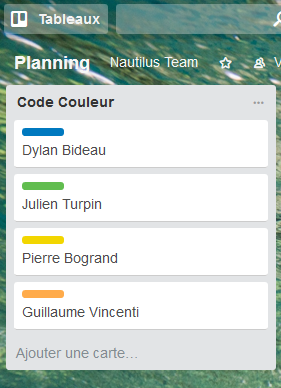
\includegraphics[scale=0.5]{Illustrations/Couleur.png}
							\end{center}
						\end{figure}
						\begin{figure}[!h]
							\paragraph{\newline Voici actuellement ce que nous devons faire : \newline}
							\begin{center}
								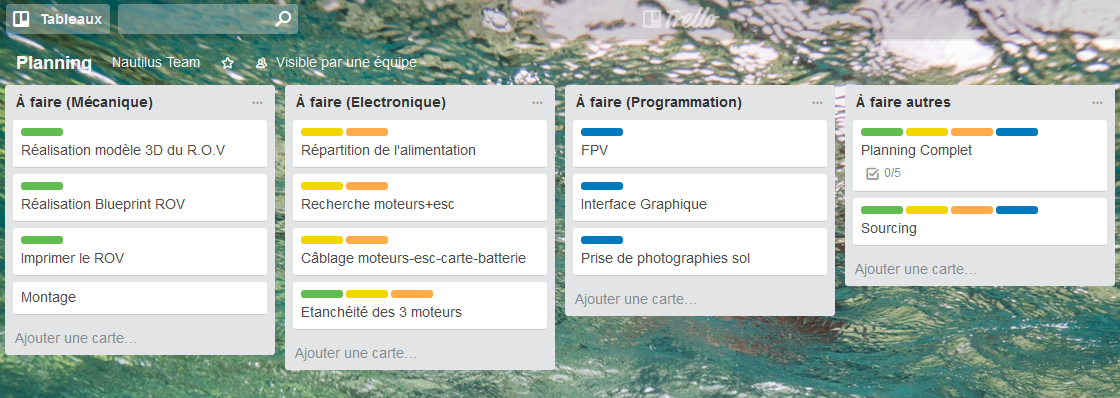
\includegraphics[scale=0.5]{Illustrations/Planning1.png}
							\end{center}
						\end{figure}
						\begin{figure}[!h]
							\paragraph{\newline Et ce que nous sommes entrain de faire ainsi que les tâches terminées : \newline}
							\begin{center}
								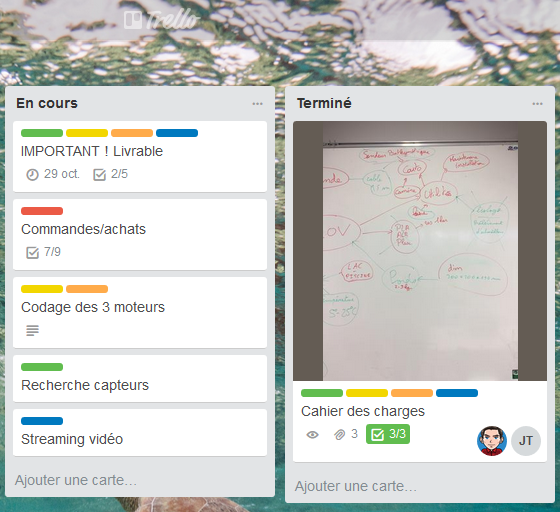
\includegraphics[scale=0.5]{Illustrations/Planning2.png}
							\end{center}
						\end{figure}
						
        \section{Github}
					\begin{figure}[!h]
							\paragraph{Tout notre code, que cela soit pour les documents en latex ou les codes liés au projet, est sur Github :\newline}
							\url{https://github.com/ROV-Nautilus/Nautilus}
							\paragraph{En voici un apercu : \newline}
							\begin{center}
								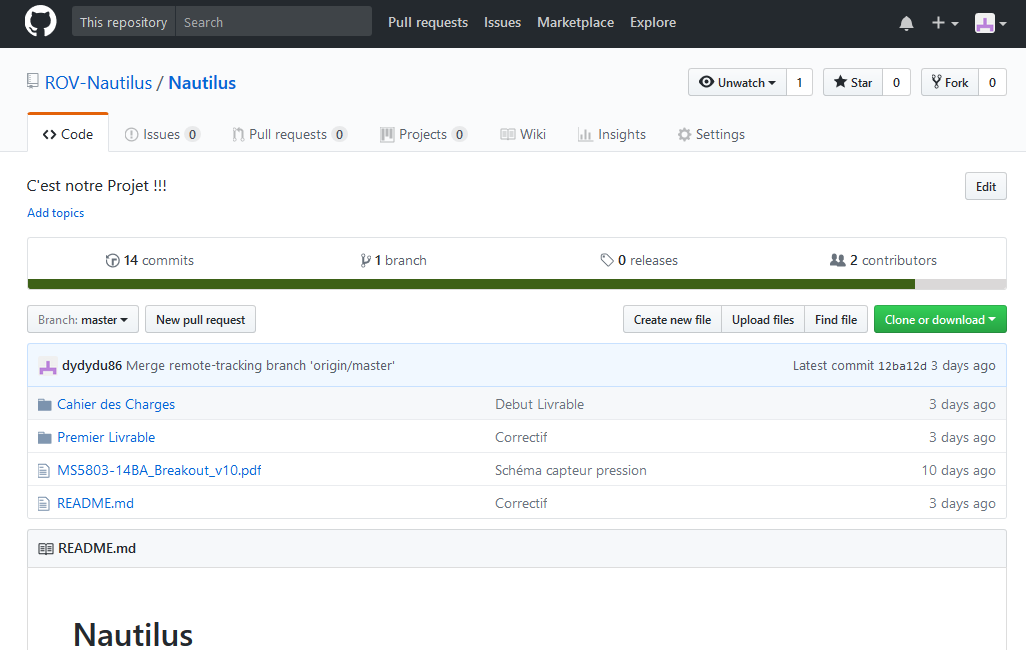
\includegraphics[scale=0.5]{Illustrations/Github.png}
							\end{center}
						\end{figure}
				
				\section{Gestion de Budget}
					\begin{figure}[!h]
							\paragraph{\newline La gestion de notre budget est réalisé à l'aide d'Excel et de Trello, en effet Trello nous permet de mettre en commun les propositions de dépenses et avec Excel nous stockons l'ensemble des commandes par fournisseurs \newline \newline Les voici ci-dessous : \newline}
							\begin{center}
								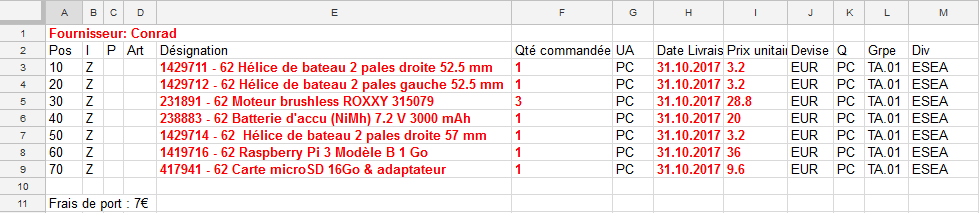
\includegraphics[scale=0.5]{Illustrations/Conrad.png}
							\end{center}
					\end{figure}
					\begin{figure}[!h]
							\begin{center}
								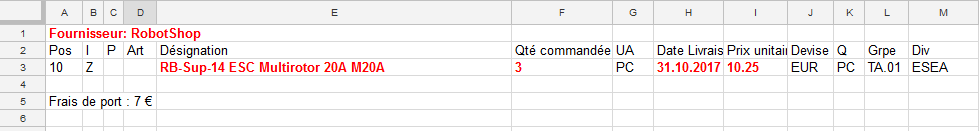
\includegraphics[scale=0.5]{Illustrations/Robotshop.png}
							\end{center}
					\end{figure}
					\begin{figure}[!h]
							\begin{center}
								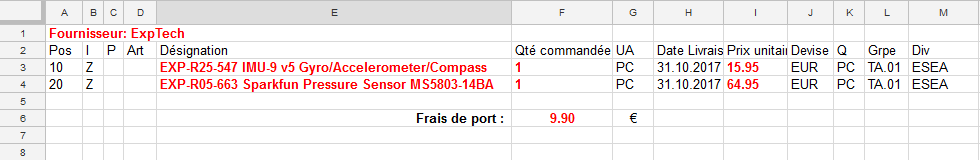
\includegraphics[scale=0.5]{Illustrations/Exptech.png}
							\end{center}
					\end{figure}

\chapter{Planning prévisionnel}
		\section{Dylan Bideau}
		\begin{center}
			\begin{tabular}{|p{3cm}|p{12cm}|}
				\hline
					\rowcolor{yellow}Dates & Travaux \\
				\hline
					7 Novembre & Stabilisation du flux des caméras en IP \newline Configurations précises des caméras \\
				\hline
					14 Novembre & Création de l'interface graphique sous python \\
				\hline
					21 Novembre \newline 28 Novembre & Amélioration de l'interface \\
				\hline
					5 Decembre \newline 19 Decembre \newline 9 Janvier & Récupération et affichage des informations des capteurs \\
				\hline
			\end{tabular}
		\end{center}
		\section{Julien Turpin}
		\begin{center}
			\begin{tabular}{|p{3cm}|p{12cm}|}
				\hline
					\rowcolor{yellow}Dates & Travaux \\
				\hline
					7 Novembre \newline 14 Novembre & Capteur de pression \\
				\hline
					21 Novembre \newline 28 Novembre \newline 5 Decembre & Matrice Inertielle \\
				\hline
					19 Decembre \newline 9 Janvier & Début conception 3D \\
				\hline
			\end{tabular}
		\end{center}
		\section{Pierre Bogrand et Guillaume Vincenti}
		\begin{center}
			\begin{tabular}{|p{3cm}|p{12cm}|}
				\hline
					\rowcolor{yellow}Dates & Travaux \\
				\hline
					7 Novembre \newline 14 Novembre & Calibration et programmation ESC \newline Test moteurs \\
				\hline
					21 Novembre \newline 28 Novembre \newline 5 Decembre & Commande moteurs \newline Ajout d'un dispositif externe de contrôle (clavier,manette) \\
				\hline
					19 Decembre \newline 9 Janvier & Etanchéité moteurs \newline Test immergé et installation \\
				\hline
			\end{tabular}
		\end{center}

\end{document}
